% !TEX TS-program = xelatex

% Use a font size of 12 point, black type. Maximum of six lines per inch. No condensed/narrow fonts, type, or spacing.
\documentclass[12pt]{article}

% set margins to CIHR standard
\usepackage[margin=2cm]{geometry}

% Uncomment this line to get six lines per inch
% \linespread{0.901} 
% See https://tex.stackexchange.com/questions/23824/6-lines-in-one-inch
% Note, I prefer to use the LaTeX default (fewer lines per inch) 
%  because it is easier to read!


\usepackage{lipsum}

%\usepackage{times}
\usepackage{mathptmx}
% use Arial font
%\usepackage{mathspec}
%\setallmainfonts(Digits,Latin)[Ligatures=TeX]{Arial}


% used to compile references into a separate PDF
\usepackage{atbegshi}


% Insert a margin of 2 cm (3/4 inch) - minimum - around the page.
\usepackage[normalem]{ulem}
\renewcommand{\ULthickness}{0.75pt}

% for rendering Figure and Table labels in bold typeface
\usepackage[labelfont=bf]{caption}


\usepackage{url}
\urlstyle{same}


%% From CIHR document:
% Indicate your name, the project title and the section title (e.g., Summary of Research Proposal) at the top of each page. 
% Indicate the page number clearly at the bottom of each page. For CV attachments, only your name (i.e., does not have to be nominated principal applicant name) and the section title (e.g., Patents and Intellectual Property Rights) are required in the header.
\usepackage{fancyhdr}

\pagestyle{fancy}
% display section title in header
\renewcommand{\sectionmark}[1]{\markright{#1}}
\renewcommand{\subsectionmark}[1]{}% Remove \subsection from header
\fancyhf{}

\renewcommand{\headrulewidth}{0.pt}
%\textheight=10in % 11in minus 2*0.5in

\lhead{\small Research Proposal}
\chead{\small Project Title}
\rhead{\small Investigator Name}
\lfoot{}
\cfoot{\thepage}
\rfoot{}


% need this to display graphics
\usepackage{graphicx}

% for putting figures and captions side-by-side in the text
\usepackage{sidecap}
\sidecaptionvpos{figure}{c}


% configure the bibliography
\usepackage[numbers,sort&compress,super]{natbib}
\makeatletter
\renewcommand{\@biblabel}[1]{#1.}
\makeatother




% section labels
\usepackage[small,compact,explicit]{titlesec}

\titleformat{\section} {\vspace{6pt}\bf\uppercase}{\thesection} {12pt} {#1\vspace{0pt}\vspace{-2pt}}

\titleformat{\subsection} {\vspace{0pt}\bf}{\thesubsection} {12pt} {\uline{#1}\vspace{-4pt}}

\titleformat{\subsubsection}[runin]{\vspace{0pt}\normalfont\normalsize\bfseries}{\thesubsubsection} {6pt} {#1}




% \titleformat{\subsubsection} [runin] {\sl}{\thesubsubsection} {8pt} {\uline{#1}}

\begin{document}

%\baselineskip 13.8pt % 1.15 * 12pt
% see http://compusavvy.wordpress.com/2010/08/01/understanding-line-and-paragraph-spacing-in-word/


%%%%%%%%%%%%%%%%%%%%%%%%%%%%%%%%%%%%%
%% From CIHR:

% Provide a clear, concise description of your research proposal, using the adjudication criteria outlined below. The research proposal should be attached as a PDF document, with a maximum of 10 pages (including figures and tables).

% The research proposal should stand alone (i.e. it should contain all the information required to support your research plan and should contain a complete description of your project).

% The research proposal may be comprised of text, tables, charts, figures and photographs, as required, and must adhere to the guidelines for attachments on the Acceptable Application Formats and Attachments.



\subsubsection * {Overview:} \lipsum[2]


\section {Concept and Significance}


\subsubsection * {First topic.}

This is how we place a literature citation\cite{Dayhoff:1983}.
The bibliography 
\lipsum[1]



\subsubsection * {Arcane but fascinating thing you don't know about.}

\lipsum[60-62]

\begin{SCfigure}[][t]
	\centering
	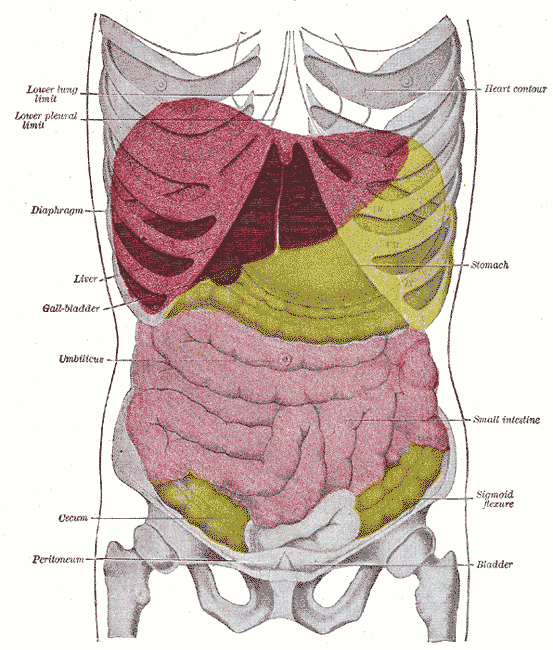
\includegraphics[width=.4\textwidth]{Gray1224}
	\caption{
	An illustration by Henry Vandyke Carter from \textit{Anatomy of the Human Body} (1918).
	This image is in the public domain and was obtained from WikiMedia Commons.}
\label{fig:model}
\end{SCfigure}






\subsubsection * {How this relates to everything you care about.}

\lipsum[8-11]


\section {Research Aims}

\lipsum[5]
Our specific aims are:
\vspace{-6pt}
\begin{enumerate}
\itemsep 0pt
\parskip 2pt
\item  To do stuff.
\item  To do other stuff that's related but independent.
\item To do even more stuff.

\end{enumerate}





\section {Approaches and Methods}


\subsection {Aim 1: The First Aim}\label{sec:aim1}

\lipsum[88]

\subsubsection {Complicated things made simple.}

\lipsum[56-59]


\subsubsection {Potential pitfalls and mitigating strategies.}

\lipsum[80-81]


\subsection {Aim 2: The Second Aim}

\lipsum[44]


\subsubsection {Preliminary results.}\label{sec:prelim}



\lipsum[40-42]


\subsubsection {Something we will do.}

Based on the preliminary work (Section \ref{sec:prelim}), we will do stuff.
\lipsum[51-53]

\subsubsection {Potential pitfalls and mitigating strategies.}

\lipsum[30]


\subsection {Aim 3: The Third Aim}

\subsubsection {Doing other things.}

\lipsum[7-11]

\subsubsection {Potential pitfalls and mitigating strategies.}

\lipsum[20]



\section {Expertise and resources}

\subsection {Expertise}\label{sec:team}

\textbf{Dr.~Science Person (Nominated Principal Applicant, 15.0 hours/week)} is a Professor of doing stuff.
They trained at the University of Here, and then went to the There Institute.
\lipsum[22]

\subsection {Resources}

\lipsum[27-28]



\newpage
\AtBeginShipout{%
\AtBeginShipoutDiscard
}

% to generate a separate PDF containing a list of references cited in this
% document, you need to compile the file `template-references.tex`
\bibliography{template}
\bibliographystyle{naturemag}

\end{document}
